\section{Case study 1: single-substrate fed-batch with a known ground truth}\label{sec:case1}

\subsection{System, library and experiments}\label{sec:c1:system}
The first case study is a single-substrate fed-batch culture with state $(X,S,V)$,
\begin{equation}
\begin{aligned}
\frac{\dd X}{\dd t} &= (\mu - k_d - D)X, \qquad \frac{\dd V}{\dd t} = F,\\
\frac{\dd S}{\dd t} &= -\frac{\mu X}{Y_{XS}} + D\,(S_{\mathrm{in}}-S),
\end{aligned}
\label{eq:c1}
\end{equation}
with $D=F/V$. The library contains eleven mechanisms (Table~\ref{tab:c1lib}): the Monod, Contois, Haldane and logistic biomass-inhibition laws, each with and without first-order death, and the Tessier, Moser and Aiba laws without death. The library is deliberately redundant. Monod, Tessier and Moser differ mainly at low substrate; Contois and Monod coincide when $K_cX\ll S$; Haldane and Aiba describe the same phenomenon, substrate inhibition, with rational and exponential forms; and a death term can be partly mimicked by a smaller yield. A twelfth, \emph{hidden} law combines Haldane substrate inhibition with logistic biomass inhibition,
\begin{equation}
\mu_{\mathrm{hidden}} = \mu_{\max}\frac{S}{K_S + S + S^2/K_I}\left(1-\frac{X}{X_{\max}}\right),
\label{eq:hidden}
\end{equation}
with $\mu_{\max}=0.6$\,h$^{-1}$, $K_S=1$\,g\,L$^{-1}$, $K_I=20$\,g\,L$^{-1}$ and $X_{\max}=30$\,g\,L$^{-1}$. Each of its ingredients is in the library, but their combination is not.

Every experiment consists of up to three 24\,h runs that differ in inoculum, initial substrate and feed (Fig.~\ref{fig:c1design}): run~a ($X_0=1$, $S_0=30$\,g\,L$^{-1}$) has a 6\,h batch phase followed by rising feed rates; run~b ($X_0=4$, $S_0=5$\,g\,L$^{-1}$) is fed from the start and stays substrate-limited at high biomass; and run~c ($X_0=0.5$, $S_0=60$\,g\,L$^{-1}$) keeps low biomass at high substrate. All runs start with $V_0=1.5$\,L and $S_{\mathrm{in}}=120$\,g\,L$^{-1}$ and are sampled 49 times, with Gaussian noise of 3\,\% of each channel's range on $X$ and $S$. Runs b and c place high biomass at low substrate and low biomass at high substrate in the same experiment, so that a rate that falls with $X$ and a rate that falls with $S$ predict different behaviour; in run~a alone, $X$ and $S$ move in opposite directions throughout (Fig.~\ref{fig:c1design}c). Each of the twelve generating laws (eleven library mechanisms and the hidden law) was simulated with the parameters of Table~\ref{tab:c1lib} for \ConeSeeds{} noise realisations. Every experiment was analysed twice, from run~a alone and from runs a--c jointly. The two analyses of an experiment took \ConeMinutes{}\,min together (median) on one CPU core.

\begin{table*}[width=\textwidth,cols=4,pos=t]
\caption{Case study 1: candidate mechanisms, parameter ranges $[\boldsymbol{\ell},\mathbf{u}]$ and true parameters of the generating models. Mechanisms marked $\pm k_d$ appear with and without death ($k_d\in[0.005,0.1]$\,h$^{-1}$, true value 0.04\,h$^{-1}$); $Y_{XS}\in[0.3,0.6]$ (true 0.5) for all. The hidden law of Eq.~\eqref{eq:hidden} is not in the library.}\label{tab:c1lib}
\begin{tabular*}{\tblwidth}{@{}LLLL@{}}
\toprule
Mechanism & $\mu(X,S)$ & Ranges & True parameters \\
\midrule
Monod $\pm k_d$ & $\mu_{\max}\,S/(K_S+S)$ & $\mu_{\max}\in[0.3,0.9]$, $K_S\in[0.1,5]$ & $\mu_{\max}=0.5$, $K_S=2$ \\
Contois $\pm k_d$ \citep{Contois1959} & $\mu_{\max}\,S/(K_cX+S)$ & $K_c\in[0.05,1]$ & $\mu_{\max}=0.5$, $K_c=1$ \\
Haldane $\pm k_d$ \citep{Andrews1968} & $\mu_{\max}\,S/(K_S+S+S^2/K_I)$ & $K_I\in[0.5,8]$ & $\mu_{\max}=0.6$, $K_S=1$, $K_I=8$ \\
Logistic $\pm k_d$ & $\mu_{\max}\,S/(K_S+S)\,(1-X/X_{\max})$ & $X_{\max}\in[12,40]$ & $\mu_{\max}=0.5$, $K_S=1$, $X_{\max}=20$ \\
Tessier \citep{Teissier1942} & $\mu_{\max}\,(1-e^{-S/K_S})$ & $K_S\in[0.1,5]$ & $\mu_{\max}=0.5$, $K_S=3$ \\
Moser \citep{Moser1958} & $\mu_{\max}\,S^{n}/(K_S+S^{n})$ & $K_S\in[0.1,25]$, $n\in[1,3]$ & $\mu_{\max}=0.5$, $K_S=16$, $n=2$ \\
Aiba \citep{Aiba1968} & $\mu_{\max}\,S/(K_S+S)\,e^{-S/K_I}$ & $K_I\in[5,50]$ & $\mu_{\max}=0.6$, $K_S=1$, $K_I=30$ \\
\bottomrule
\end{tabular*}
\end{table*}

\begin{figure*}
\centering
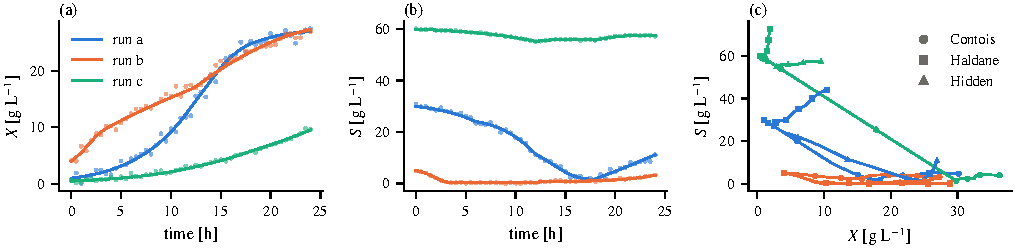
\includegraphics[width=\textwidth]{figs/c1_design.pdf}
\caption{Case study 1, experiment design (hidden law, first noise realisation). (a) Biomass and (b) substrate in the three runs; points are measurements, lines the noise-free trajectories. (c) The three runs in the $X$--$S$ plane for three generating laws: in run~a (blue) biomass and substrate move in opposite directions, whereas runs b and c reach high biomass at low substrate and low biomass at high substrate.}
\label{fig:c1design}
\end{figure*}

The symbolic-regression dictionary for $\mu$ contains the numerator terms $\{S,\ SX,\ S^2,\ S\,e^{-S/K}\}$ and the denominator terms $\{1,\ X,\ S^2,\ SX\}$, with laws of up to four terms. In the form of Eq.~\eqref{eq:sr}, Monod corresponds to $\{S;\,1\}$, Contois to $\{S;\,X\}$, Haldane to $\{S;\,1,S^2\}$, the logistic law to $\{S,SX;\,1\}$, Tessier to $\{S,\,S e^{-S/K}\}$, Aiba to $\{S e^{-S/K};\,1\}$, and the hidden law to $\{S,SX;\,1,S^2\}$. Moser, with a non-integer exponent, cannot be expressed.

\subsection{The hybrid model learns the kinetics}\label{sec:c1:node}
Figure~\ref{fig:c1mu} compares the specific growth rates learned by the hybrid model with the true ones along run~a. Without being told the mechanism, the network reproduces each law's signature: the abrupt drop of Monod, Tessier and Moser growth when the batch substrate is exhausted, the gradual decline of Contois and logistic growth as biomass accumulates, and the \emph{rise} of the Haldane and Aiba rates as an inhibitory substrate is consumed. The median training loss was \ConeNodeLossSingle{} on single runs, at the noise floor of $0.03^2\approx 9\times10^{-4}$ implied by Eq.~\eqref{eq:loss}, and \ConeNodeLossJoint{} on three runs, where one network must describe three regimes at once. The learned rates are therefore an accurate but not a perfect reference; the selection never relies on them alone.

\begin{figure*}
\centering
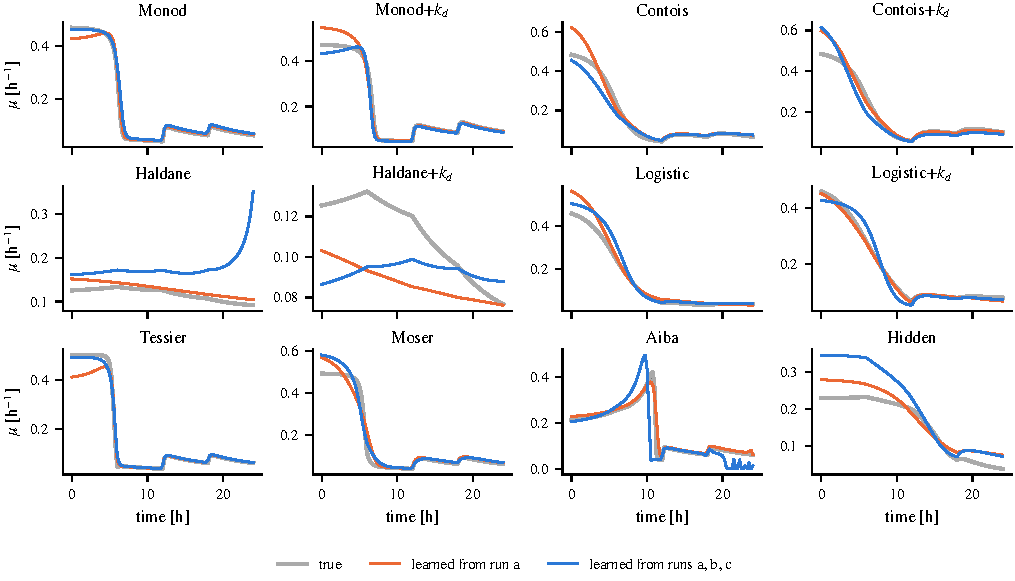
\includegraphics[width=\textwidth]{figs/c1_learned_mu.pdf}
\caption{Specific growth rate along run~a: true (grey) and learned by the hybrid neural ODE from run~a alone (orange) or from runs a--c jointly (blue), for the twelve generating laws (first noise realisation).}
\label{fig:c1mu}
\end{figure*}

The substrate factor in Eq.~\eqref{eq:rate} is essential when the culture becomes substrate-limited (Table~\ref{tab:ablation}). With a softplus output alone, the network assigns a positive growth rate at zero substrate; in the Monod experiment, which is substrate-limited for most of its duration, the model then drives the substrate below zero and the training loss and the error of the learned rate both increase several-fold. Runs whose substrate never falls near zero (Haldane) are unaffected.

\begin{table}[width=\linewidth,cols=7,pos=t]
\caption{Effect of the substrate factor $S/(S+K)$ in Eq.~\eqref{eq:rate}: medians over \ConeSeeds{} noise realisations of run~a. Loss in units of $10^{-3}$; rate error is the root-mean-square error of the learned $\mu$ relative to the maximum true $\mu$; $S_{\min}$ is the lowest substrate concentration of the trained model.}\label{tab:ablation}
\begin{tabular*}{\tblwidth}{@{}LCCCCCC@{}}
\toprule
 & \multicolumn{2}{c}{Loss} & \multicolumn{2}{c}{Rate error} & \multicolumn{2}{c}{$S_{\min}$ [g\,L$^{-1}$]} \\
Generating law & with & without & with & without & with & without \\
\midrule
\inputtab{generated/tab_c1_ablation.tex}
\bottomrule
\end{tabular*}
\end{table}

\subsection{Selection from one run is ambiguous}\label{sec:c1:single}
Table~\ref{tab:c1sel} and Fig.~\ref{fig:c1conf}a summarise the selection from run~a alone. With the four basic mechanisms as the library, the generating mechanism was selected in \ConeAccFour\,\% of the cases; with the full library of eleven, in \ConeAccSingle\,\%, with a mean BIC weight of \ConeWtrueSingle{} on the true mechanism and the true mechanism on the shortlist in \ConeShortSingle\,\%. Every best fit passed the adequacy test, so the errors are not failures of the fitting but ambiguities of the data. They follow the structure of the library. Monod, Tessier, Moser and Contois share the weight, because they differ mainly in the brief low-substrate window that a fed-batch run crosses quickly. Haldane is read as Contois or Aiba: along run~a the substrate falls while biomass rises, so a growth rate that changes because $S$ falls cannot be told apart from one that changes because $X$ rises. Aiba and Haldane+$k_d$ are confused with each other, as two forms of substrate inhibition. Death variants are partly confused with their death-free counterparts.

\begin{table}[width=\linewidth,cols=6,pos=t]
\caption{Case study 1: selection accuracy [\%] and mean BIC weight of the generating mechanism over \ConeSeeds{} noise realisations, from run~a alone with the four-mechanism and the eleven-mechanism library, and from runs a--c jointly with the eleven-mechanism library.}\label{tab:c1sel}
\tabcolsep=3.5pt
\begin{tabular*}{\tblwidth}{@{}LCCCCC@{}}
\toprule
 & 4 mech. & \multicolumn{2}{c}{11 mech., run a} & \multicolumn{2}{c}{11 mech., runs a--c} \\
Generating law & acc. & acc. & weight & acc. & weight \\
\midrule
\inputtab{generated/tab_c1_selection.tex}
\bottomrule
\end{tabular*}
\end{table}

\subsection{Three jointly fitted runs resolve the ambiguity}\label{sec:c1:joint}
Fitting runs a--c jointly, with shared kinetic parameters and one initial state per run, removes the ambiguity (Fig.~\ref{fig:c1conf}b): the generating mechanism was selected in \ConeAccJoint\,\% of the \ConeLibCasesJoint{} library cases, with a mean weight of \ConeWtrueJoint{}. The remaining weight sits on nested alternatives with one extra parameter (a death term, or the Moser exponent). The two additional runs do not add new kinds of measurements; they add operating points at which the candidates make different predictions. Haldane, for example, is identified because run~c keeps the substrate in the inhibitory range at low biomass, where a Contois or logistic law predicts fast growth.

\begin{figure*}
\centering
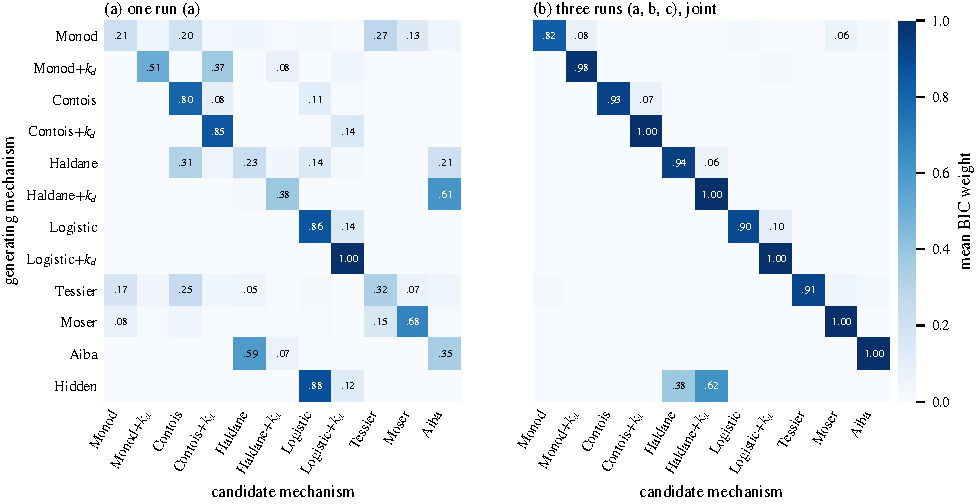
\includegraphics[width=\textwidth]{figs/c1_confusion.pdf}
\caption{Case study 1: mean BIC weight of every candidate (columns) for every generating law (rows) over \ConeSeeds{} noise realisations, (a) from run~a alone and (b) from runs a--c jointly. The last row is the hidden law, which is not in the library.}
\label{fig:c1conf}
\end{figure*}

\subsection{Symbolic regression: no false discoveries, non-rational laws recovered}\label{sec:c1:sr}
Symbolic regression proposed seven laws per analysis, which were refined with and without a death term and ranked together with the library. Figure~\ref{fig:c1sr} shows, for every analysis, the BIC difference between the best proposed law and the best library mechanism. For the eleven library experiments the proposed laws never met the acceptance rule (\ConeFalseDiscSingle{} of \ConeLibCasesSingle{} single-run and \ConeFalseDiscJoint{} of \ConeLibCasesJoint{} joint analyses): when the generating law is in the library, the regression does not produce spurious discoveries. In many of these cases the best proposed law \emph{is} the library law written in the form of Eq.~\eqref{eq:sr} and ties with it ($\Delta\BIC\approx 0$; Table~\ref{tab:c1sr}). This includes the two non-rational laws: the exponential dictionary term recovered the Aiba structure in \ConeAibaRedisc\,\% and the Tessier structure in \ConeTessierRedisc\,\% of the joint analyses. Moser, which the dictionary cannot express, was always better described by its library entry ($\Delta\BIC\approx 95$).

\begin{table}[width=\linewidth,cols=3,pos=t]
\caption{Case study 1, symbolic regression on runs a--c jointly: frequency [\%] with which the generating structure was among the proposed laws within two BIC units of the best one, and median BIC difference between the best proposed law and the best library mechanism (positive: the library mechanism is preferred).}\label{tab:c1sr}
\begin{tabular*}{\tblwidth}{@{}LCC@{}}
\toprule
Generating law & Structure recovered & Median $\Delta\BIC$ \\
\midrule
\inputtab{generated/tab_c1_sr.tex}
\bottomrule
\end{tabular*}
\end{table}

\begin{figure*}
\centering
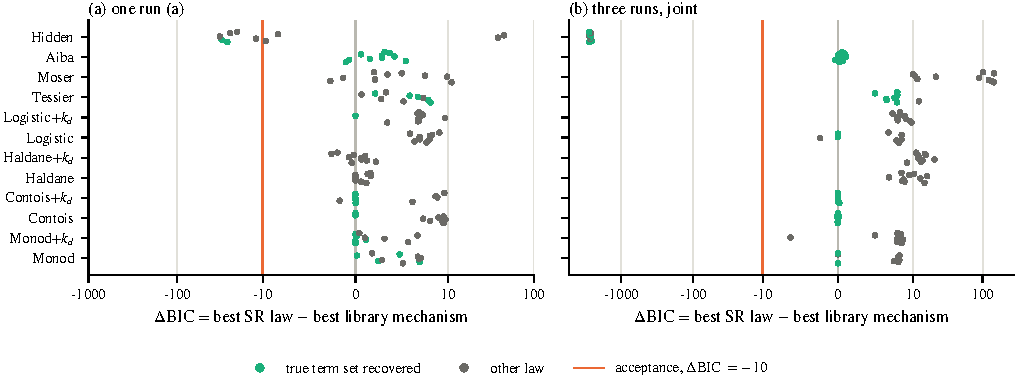
\includegraphics[width=\textwidth]{figs/c1_sr.pdf}
\caption{Case study 1: BIC difference between the best law proposed by symbolic regression and the best library mechanism, for every generating law and noise realisation, (a) from run~a alone and (b) from runs a--c jointly (symmetric logarithmic axis). Green: the generating structure is among the proposed laws within two BIC units of the best one. The orange line marks the acceptance threshold $\Delta\BIC=-10$; only the hidden law crosses it.}
\label{fig:c1sr}
\end{figure*}

\subsection{A mechanism missing from the library}\label{sec:c1:hidden}
For the hidden law the behaviour depends on the data. From run~a alone the best library mechanism, the logistic law, fits within the noise (median $\chi^2=\ConeHiddenChiLibSingle$ against the adequacy limit of \ConeChiOKsingle{} for $n=98$), so nothing indicates that the library is incomplete. Symbolic regression nevertheless proposed a better law in \ConeHiddenBestSingle{} of \ConeHiddenN{} realisations and one that met the acceptance rule in \ConeHiddenAcceptedSingle{}, but the proposed structure was the true one in only \ConeHiddenFoundSingle{}. A single run thus contains evidence that the library is missing something, but not enough to say what.

With three runs the picture changes (Fig.~\ref{fig:c1hidden}). The best library mechanism, now Haldane, fails the adequacy test in \ConeHiddenFlagJoint{} of \ConeHiddenN{} realisations (median $\chi^2=\ConeHiddenChiLib$ against a limit of \ConeChiOK{} for $n=294$), which triggers the escalation: all \ConeScreened{} admissible laws are screened against the measurements and the five best are refined. The best law then fits within the noise (median $\chi^2=\ConeHiddenChiSR$) and is accepted in \ConeHiddenAcceptedJoint{} of \ConeHiddenN{} realisations. Its structure is exactly that of the hidden law, $\{S,SX;\,1,S^2\}$, in \ConeHiddenFoundJoint{} realisations; in the other \ConeHiddenEquivJoint{}, the numerator term $S$ is replaced by $S\,e^{-S/K}$ with $K$ between \ConeHiddenKmin{} and \ConeHiddenKmax{}\,g\,L$^{-1}$, a factor between 0.86 and 1 over the observed substrate range, i.e.\ the same law for all practical purposes. For the first realisation the discovered law, rewritten in the conventional form, is
\begin{equation}
\mu = \ConeHidMumax\,\frac{S\,\big(1 - X/\ConeHidXmax\big)}{\ConeHidKs + S + S^2/\ConeHidKi},
\label{eq:discovered}
\end{equation}
against the true $\mu_{\max}=0.6$\,h$^{-1}$, $X_{\max}=30$, $K_S=1$ and $K_I=20$\,g\,L$^{-1}$.

The escalation was necessary. The true structure was never among the laws shortlisted by their match to the learned rates (\ConeHiddenShortTrue{} of \ConeHiddenN{} realisations), and the best shortlisted law passed the adequacy test in only \ConeHiddenPreOK{}. The reason is the accuracy of the learned rate: along run~a it deviated from the true rate by up to \ConeHiddenErrAmax\,\% of its maximum (median \ConeHiddenErrAmed\,\%), against at most \ConeHiddenErrBCmax\,\% along runs b and c. With errors of this size, a wrong law can match the learned rate better than the true one. The screening against the measurements does not depend on the learned rates and corrects this.

\begin{figure*}
\centering
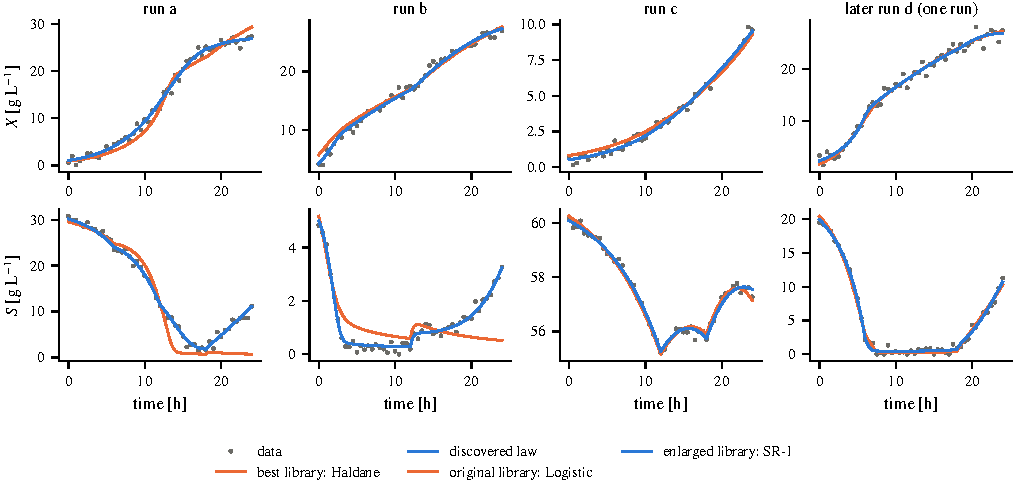
\includegraphics[width=\textwidth]{figs/c1_hidden.pdf}
\caption{Hidden law (first noise realisation). Runs a--c: measurements, best library mechanism (Haldane, orange) and the law discovered after escalation (blue), all fitted jointly. Later run d: a single new run analysed with the original library (orange; best: logistic) and with the library enlarged by the discovered law (blue).}
\label{fig:c1hidden}
\end{figure*}

\paragraph{Closing the loop}
The accepted law was added to the library (as ``SR-1'') and the enlarged library was used, without symbolic regression, on a later single run under new conditions (run~d: $X_0=2$, $S_0=20$\,g\,L$^{-1}$, $S_{\mathrm{in}}=150$\,g\,L$^{-1}$, a different feed). With the original library the logistic law was selected in \ConeLaterBaseCount{} of \ConeLoopN{} realisations. With the enlarged library, SR-1 fitted run~d better than every original mechanism in \ConeLaterBetterChi{} realisations (by up to \ConeLaterDchiMax{} $\chi^2$ units) and was selected with a weight above 0.9 in \ConeLaterStrong{}; in the others the logistic law, with one parameter fewer, was preferred. Run~d never exceeds about 20\,g\,L$^{-1}$ of substrate, where the inhibition term of the hidden law is weak, so a single run in this regime gives only moderate evidence for it; the library entry nevertheless makes the better law available. Conversely, refined on the eleven library experiments, SR-1 never took more than \ConeStealMax{} of the BIC weight and did not change any selection (\ConeStealChanged{} of \ConeStealCases{}): enlarging the library did not compromise the identification of the existing mechanisms.
